\documentclass[11pt]{article}
\usepackage[T1]{fontenc}
\usepackage{bookmark}
\usepackage{tocloft}
\usepackage{graphicx}
\usepackage{booktabs}
\usepackage{subcaption}
\usepackage[a4paper, total={6in, 9in}]{geometry}

\graphicspath{{../tutorial/}{../db_schema/}{../json/}{../sql_nosql/mongodb/screenshots/}}

\title{\textbf{Benchmark baz danych}}
\author{Aleks Zieliński, Filip Kalinowski}
\date{\today}

\hypersetup{hidelinks}
\renewcommand\contentsname{\hfill\bfseries\Large Rozdziały \hfill}
\renewcommand{\cftaftertoctitle}{\hfill}
\DeclareCaptionFormat{custom}
{%
    \textbf{#1#2}\textit{\small #3}
}
\captionsetup{format=custom}
\renewcommand{\figurename}{Zdjęcie.}

\begin{document}
\maketitle

\newpage
\begingroup
\tableofcontents
\endgroup

\newpage
\section{Informacje wstępne}
	\subsection{Założenia projektu}
		\begin{enumerate}
			\item Zaprojektować schemat dokumentów JSON dla wybranego tematu. Należy mieć min 2 typy dokumentów na osobę w projekcie. Minimum jeden typ musi mieć dokumenty zagnieżdżone
			\item  Opracowany model, wraz z propozycją najważniejszych/najbardziej rozbudowanych poleceń należy zatwierdzić u wykładowcy (ew. poprawić wg. sugestii)
			\item Dla każdego typu dokumentu wygenerować min 100 sensownych instancji. Jeden z typów powinien mieć minimum 500 instancji. Dane można generować automatami typu generatedata.com bądź napisać 4 skrypt w pythonie (dodatkowe punkty).
			\item  Tak przygotowane dokumenty należy zaimportować do:
			\begin{itemize}
				\item Wybranej bazy NoSQL
				\item PostgreSQLa do kolumn typu JSONB
				\item PostgreSQLa przy jednoczesnej konwersji JSON na tabele
			\end{itemize}
			\item Wszystkie 3 procesy importowania należy udokumentować screenshotami i zapisanymi wykorzystanymi poleceniami
			\item  Należy utworzyć min 4 zapytania na osobę realizujące najważniejsze problemy wyszukiwania w tworzonej bazie. 
			\item Każde z zapytań musi mieć 3 wersje dla 3 sytuacji z pkt 4. 
			\item Należy przeprowadzić eksperyment pomiaru czasu wykonania tych zapytań. Aby eksperyment był rzetelnie przeprowadzony, zarówno baza NoSQLowa, jak i PostgreSQL muszą operować w podobnych warunkach: albo obie bazy są postawione w osobnych dockerach, albo zainstalowane w tym samym OS, ale uruchamiane jedna na raz (proces instalacji musi być udokumentowany). Wyniki czasowe należy przedstawić w tabelce
		\end{enumerate}
	\subsection{Użyte technologie i sprzęt}
		\begin{itemize}
			\item PostgreSQL - wersja 16.9
			\item MongoDB - wersja 8.0.10
			\item Laptop:
			\begin{itemize}
				\item OS - Linux Mint 22.1
				\item CPU - Intel i7-9750H
				\item GPU - Nvidia GTX 1660
				\item RAM - 16GB 2667 MHz		
			\end{itemize}
		\end{itemize}
	
\newpage
	\subsection{Schemat logiczny bazy danych}
		\begin{figure}[!ht]
			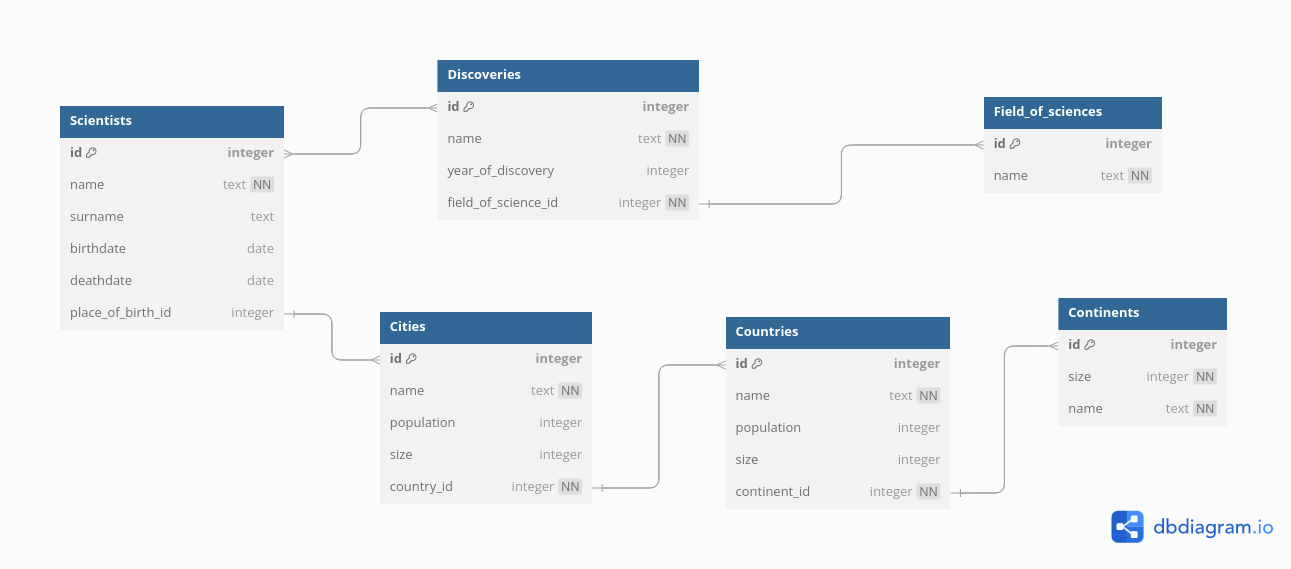
\includegraphics[width=\textwidth]{db-bench.png}
			\caption{Schemat logiczny zrobiony w serwisie dbdiagram.io}
		\end{figure}
	\subsection{Przykładowe dane z plików JSON}
		\begin{figure}[!ht]
			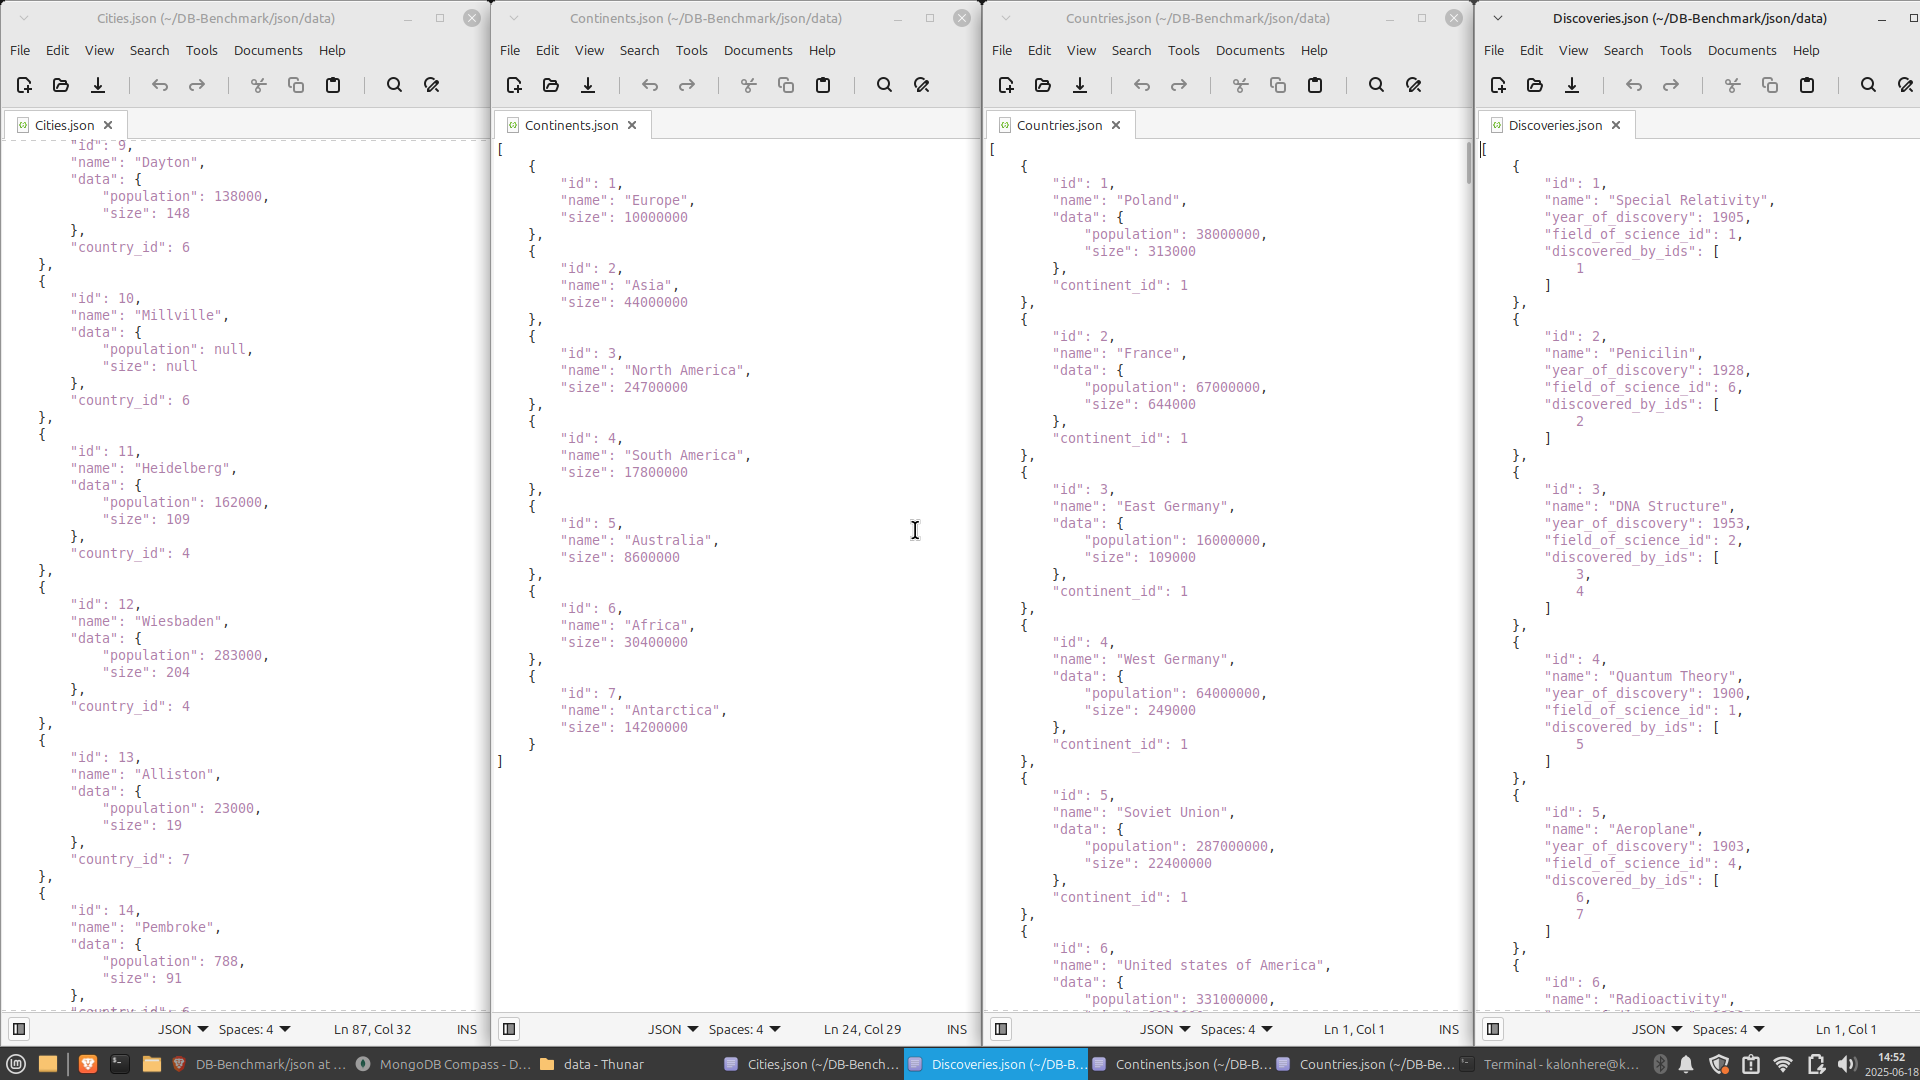
\includegraphics[width=\textwidth]{JSON_examples_1.png}
			\caption{Pliki JSON od lewej: Cities, Continents, Countries, Discoveries}
		\end{figure}

\newpage
		\begin{figure}[!ht]
			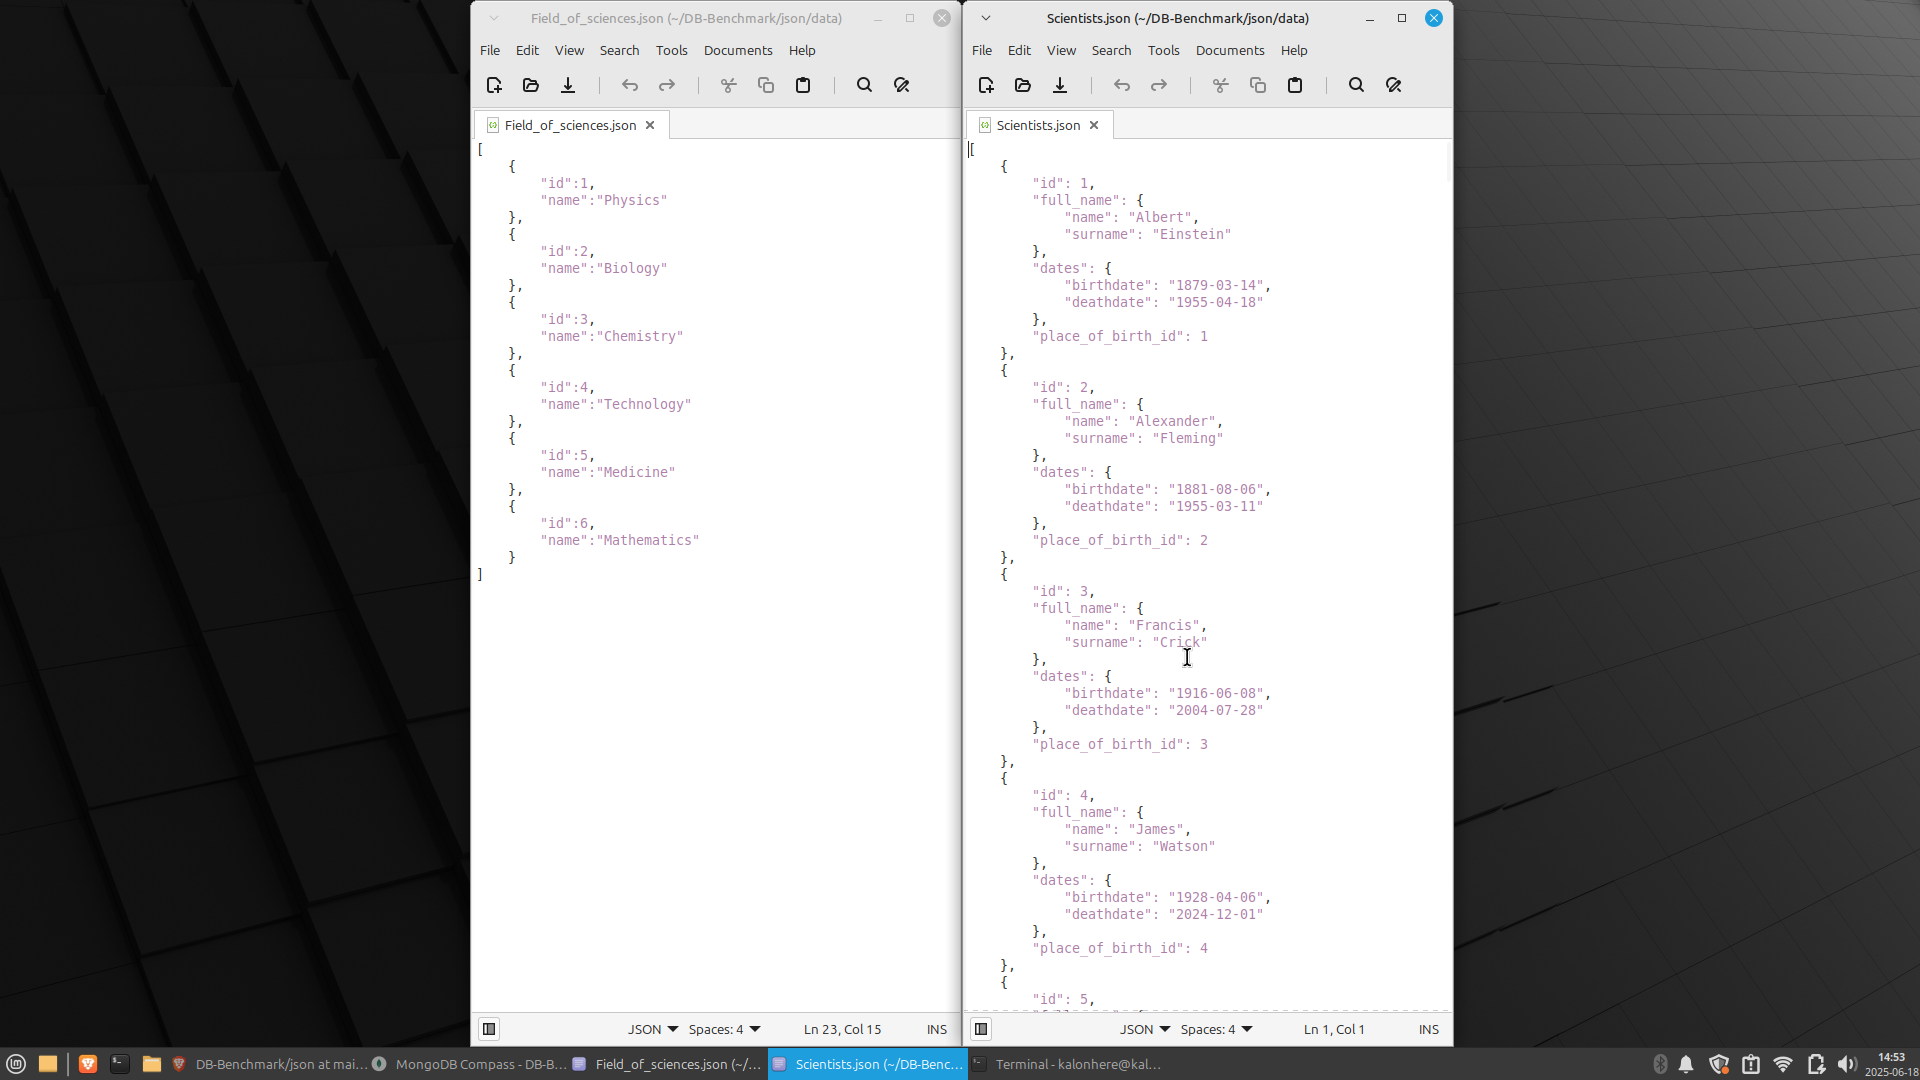
\includegraphics[width=\textwidth]{JSON_examples_2.png}
			\caption{Pliki JSON od lewej: Field\_of\_sciences, Scientists}
		\end{figure}
\section{Instalacja baz danych}
	\subsection{PostgreSQL}
		\begin{figure}[!ht]
			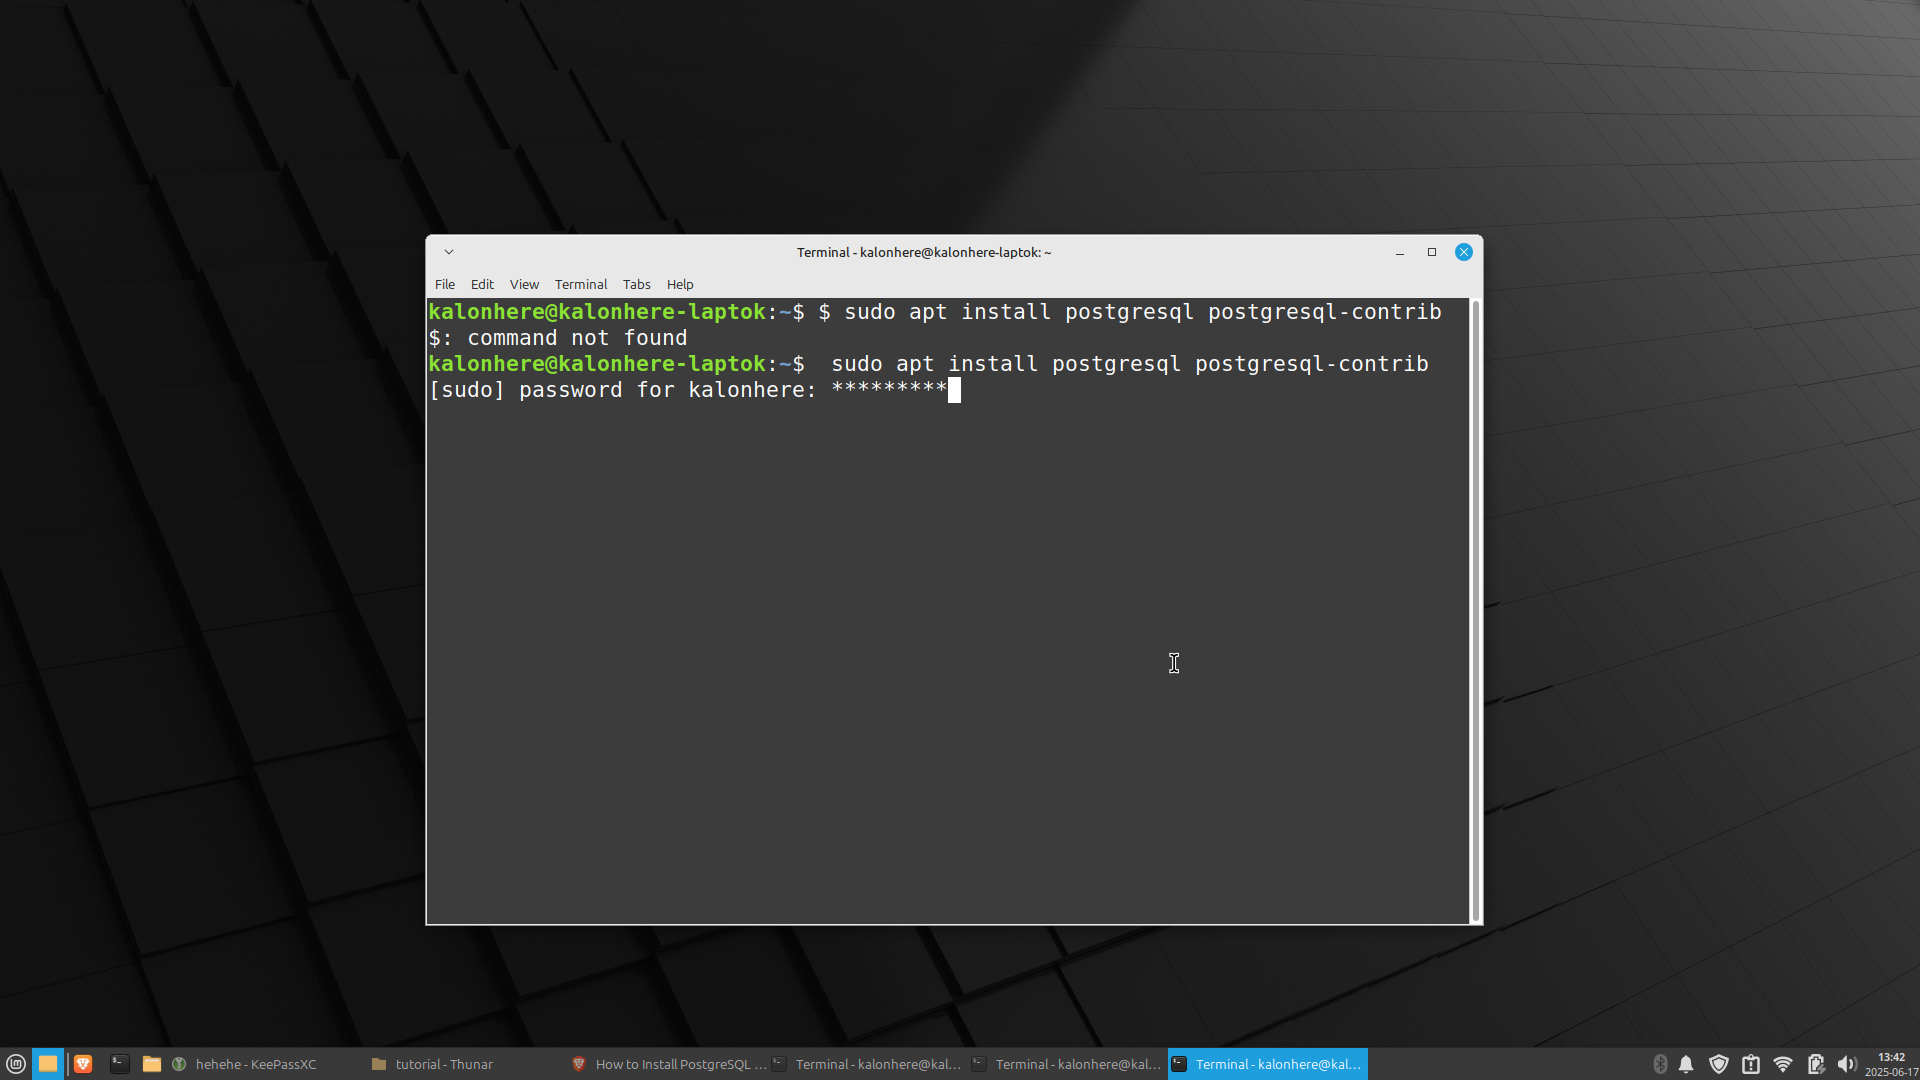
\includegraphics[width=\textwidth]{1_instalacja_postgresa.png}
			\caption{Instalacja za pomocą apt}
		\end{figure}
		\begin{figure}[!ht]
			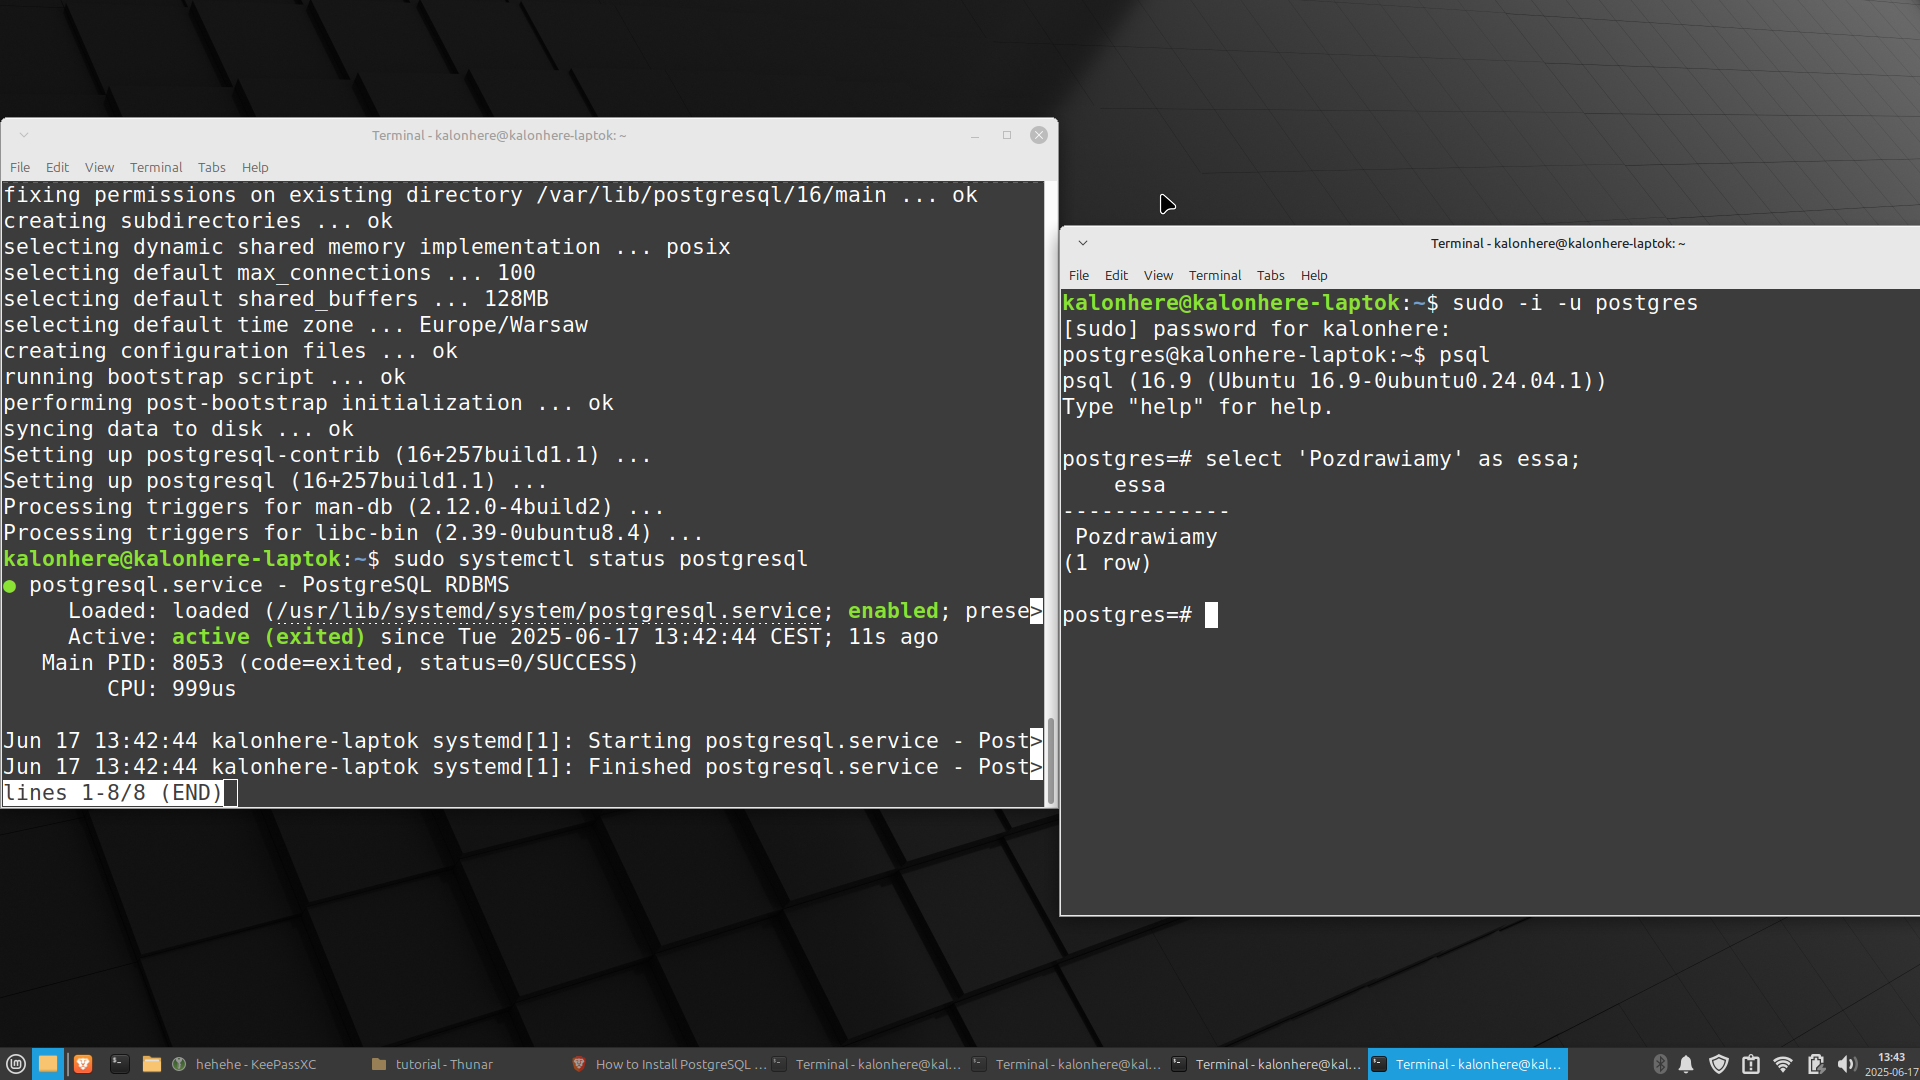
\includegraphics[width=\textwidth]{2_sprawdzenie_postgresa_i_psql.png}
			\caption{Po lewej - komenda systemctl aby sprawdzić czy działa, po prawej - logowanie na user, uruchomienie psqgl i test działania}
		\end{figure}

\newpage
		\begin{figure}[!ht]
			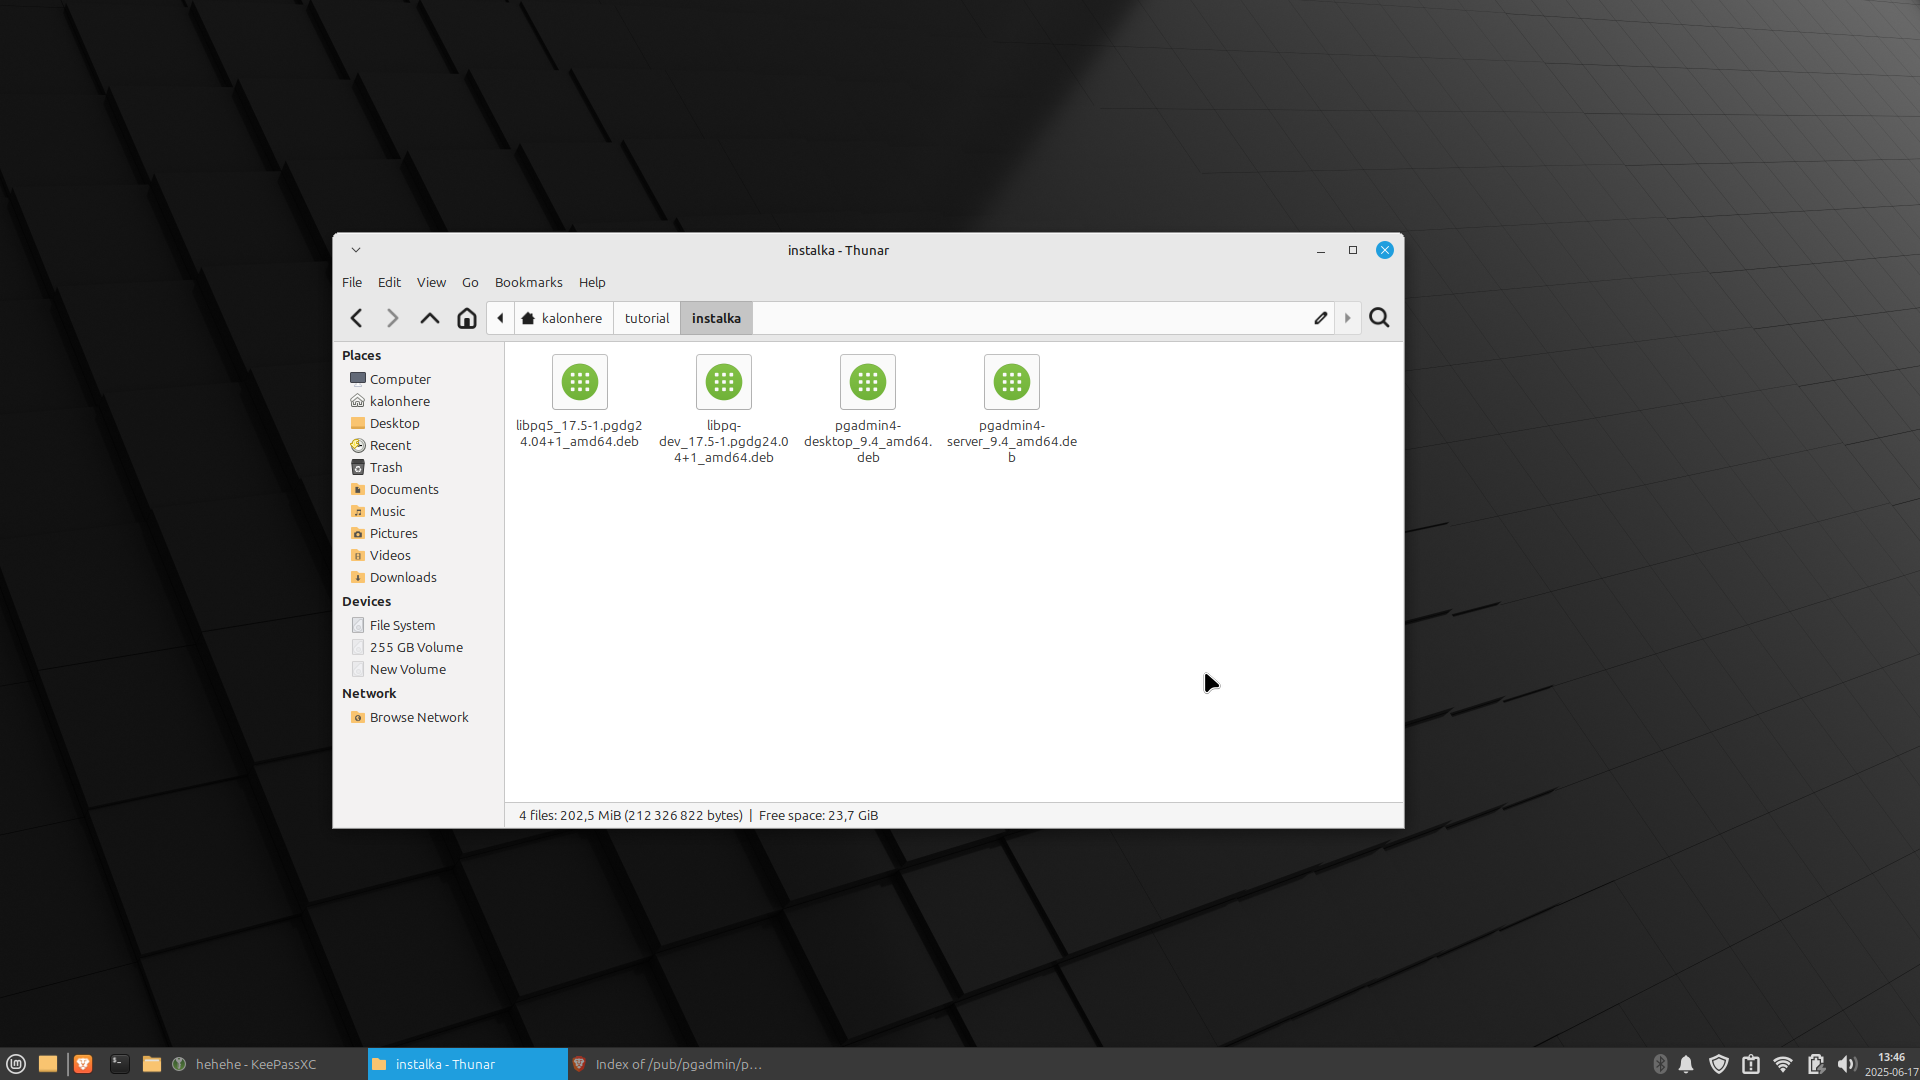
\includegraphics[width=\textwidth]{3_instalacja_pgadmin_wiem_co_robie.png}
			\caption{Instalacja pgadmina z serwera ftp PostgreSQL}
		\end{figure}

\newpage
	\subsection{MongoDB}
		\begin{figure}[!ht]
			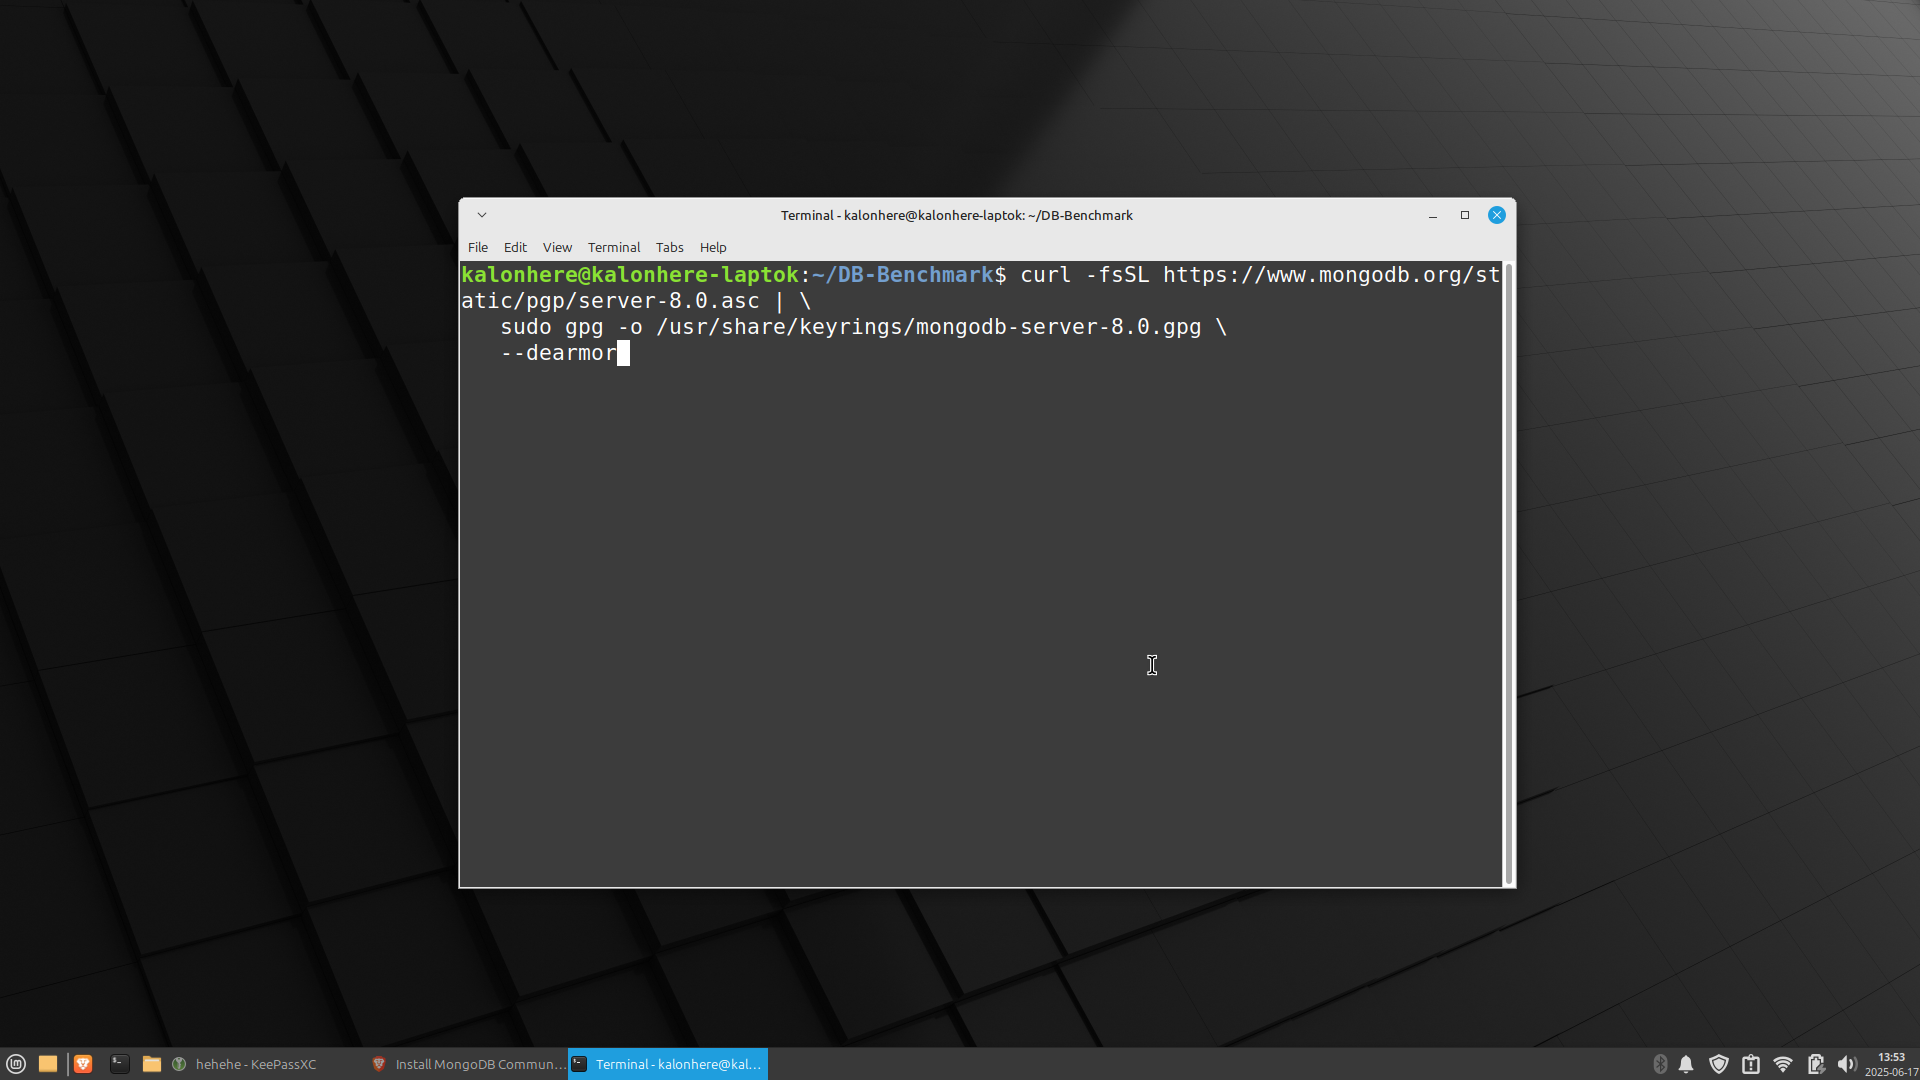
\includegraphics[width=\textwidth]{4_importowanie_klucza_gpg.png}
			\caption{Importowanie kluczy gpg do MongoDB}
		\end{figure}
		\begin{figure}[!ht]
			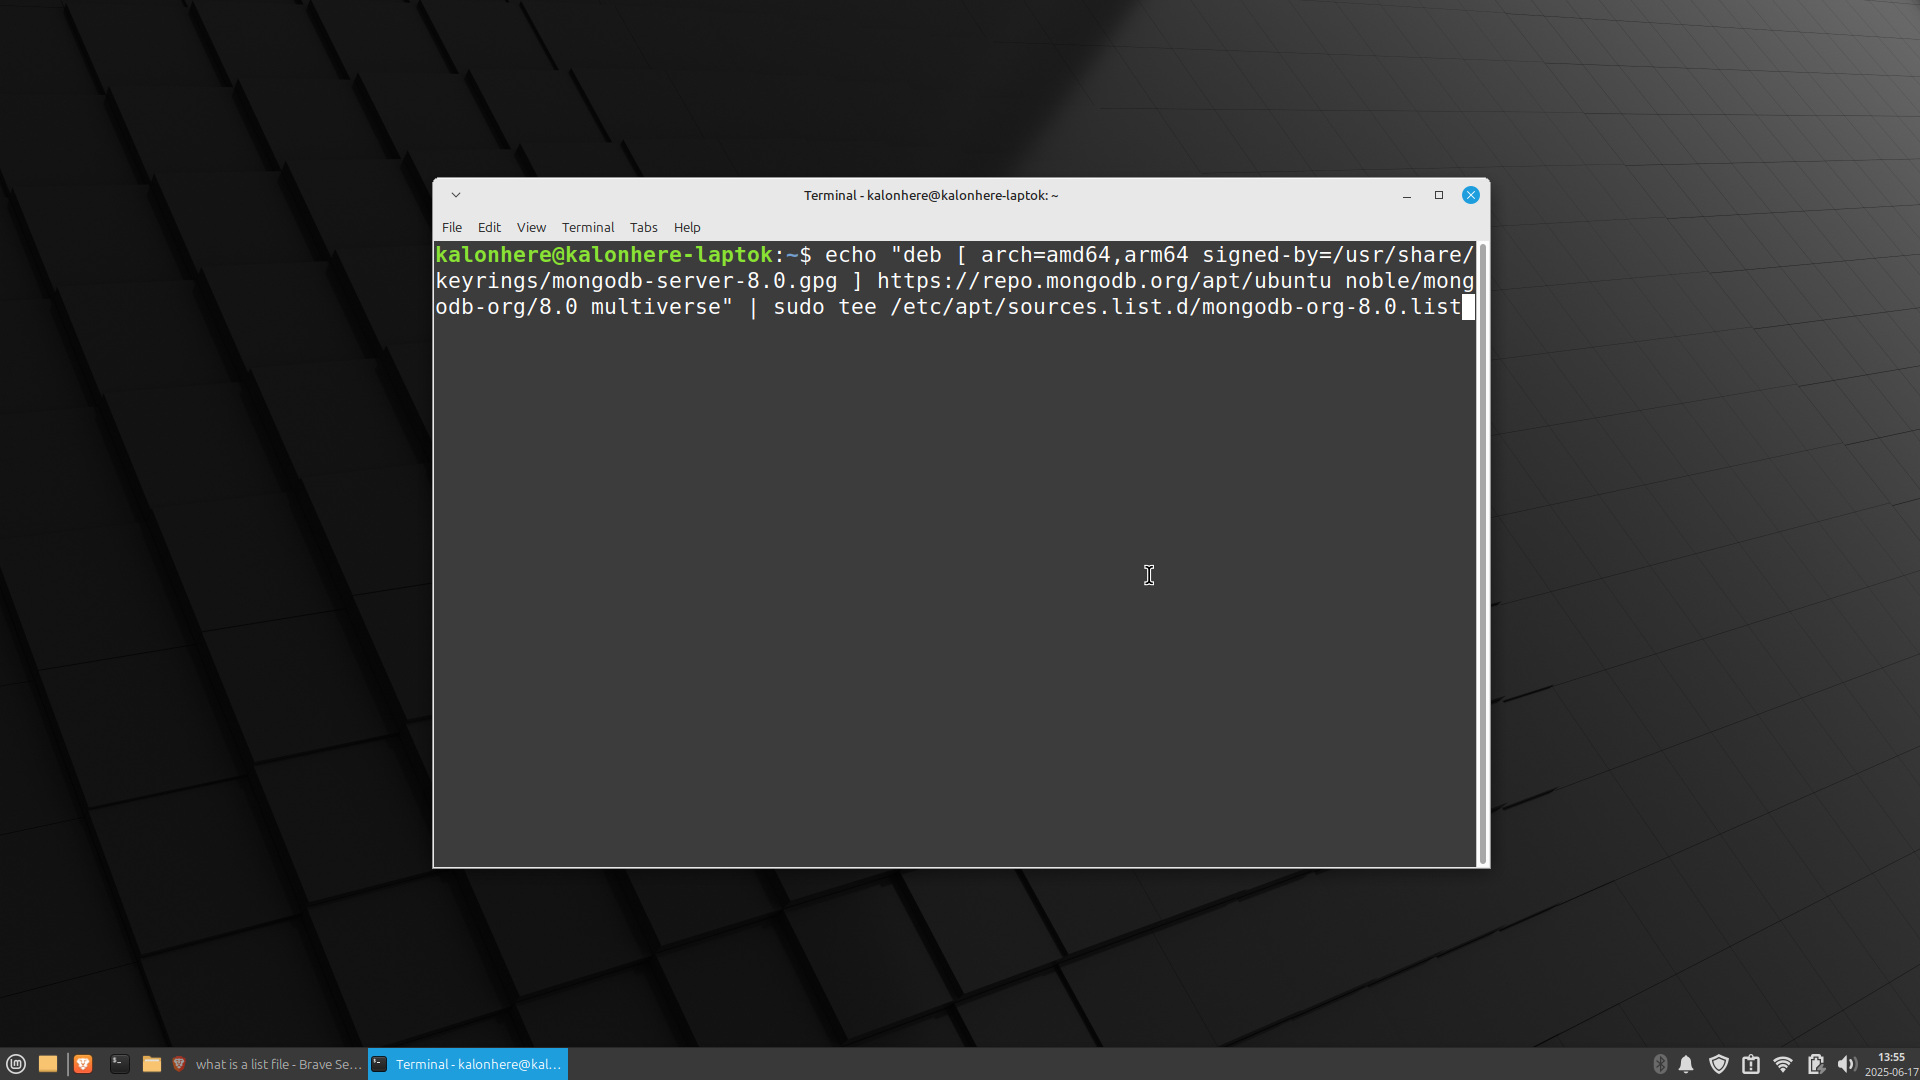
\includegraphics[width=\textwidth]{5_tworzenie_pliku_z_listami_source_do_repo.png}
			\caption{Stworzenie pliku z listą źródeł do pobierania repo/package}
		\end{figure}

\newpage
		\begin{figure}[!ht]
			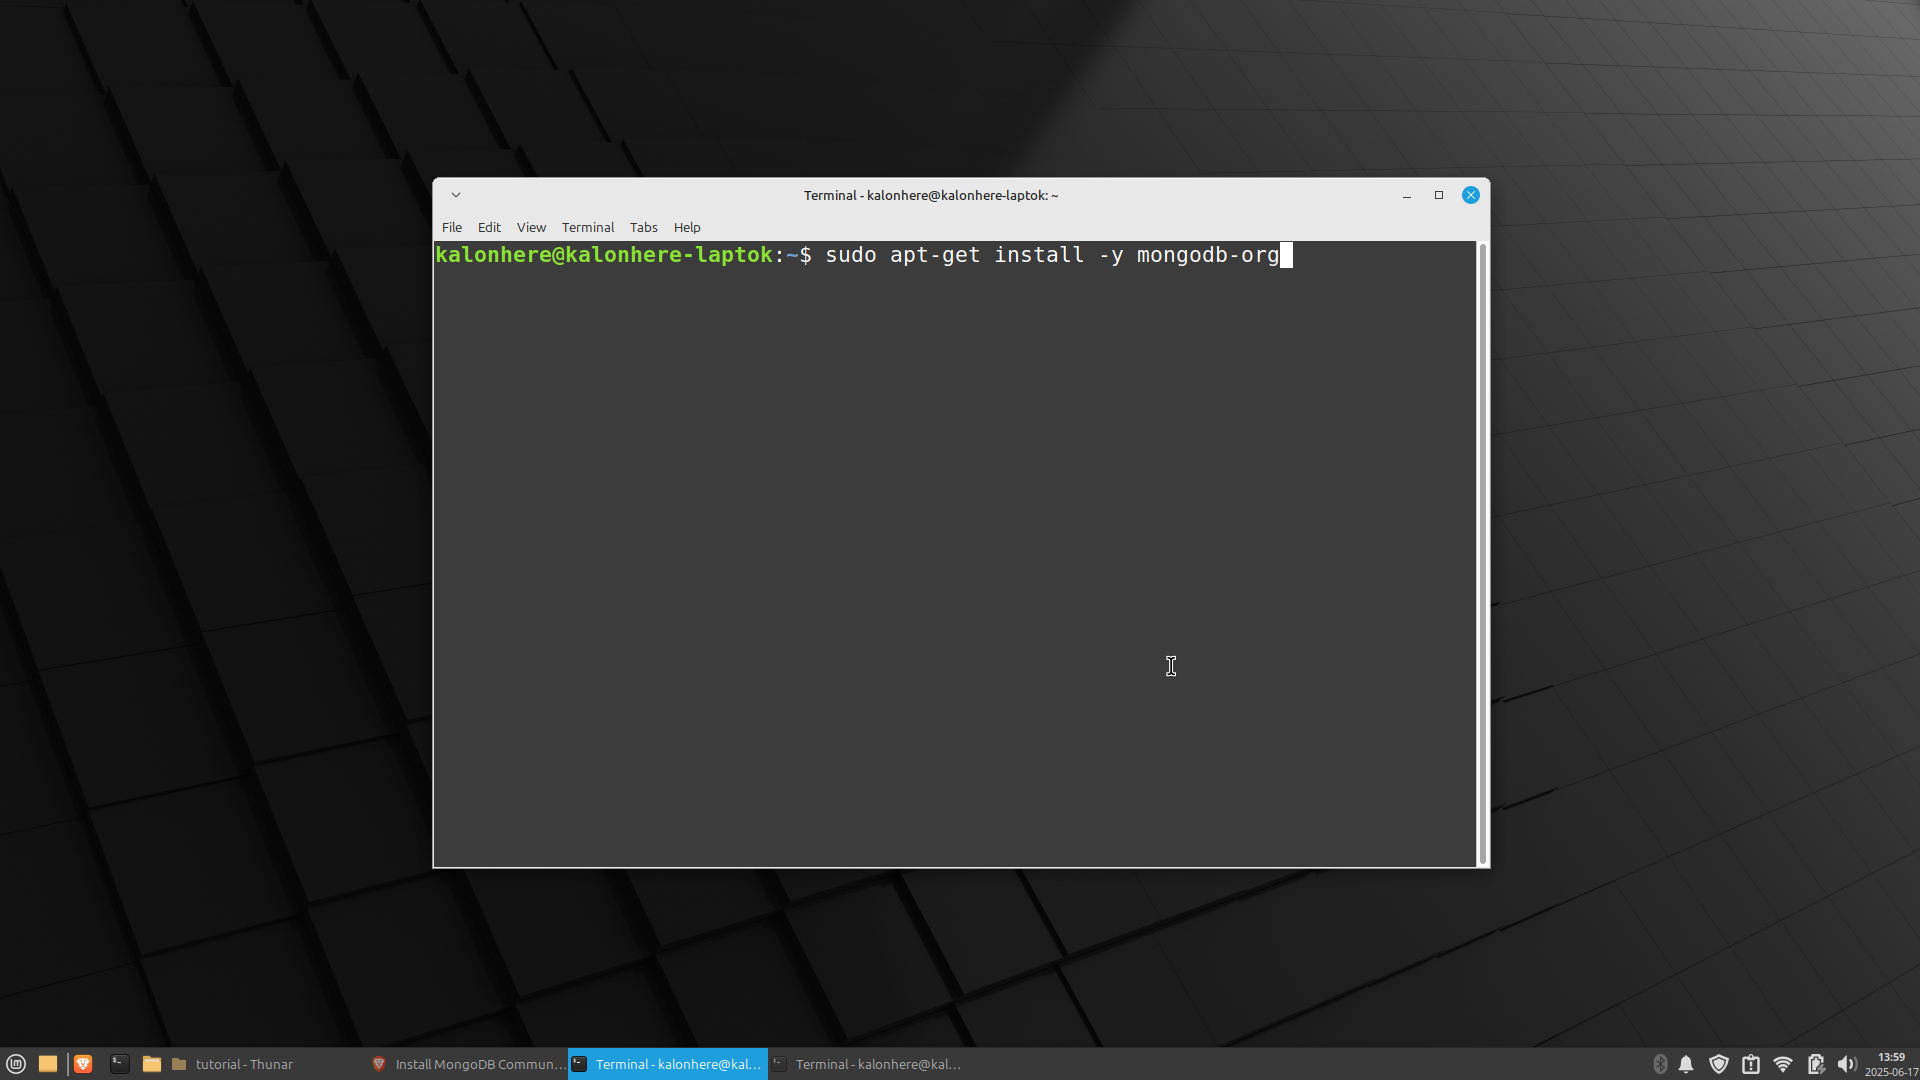
\includegraphics[width=\textwidth]{6_instalacja_mongodb.png}
			\caption{Instalacja MongoDB}
		\end{figure}
		\begin{figure}[!ht]
			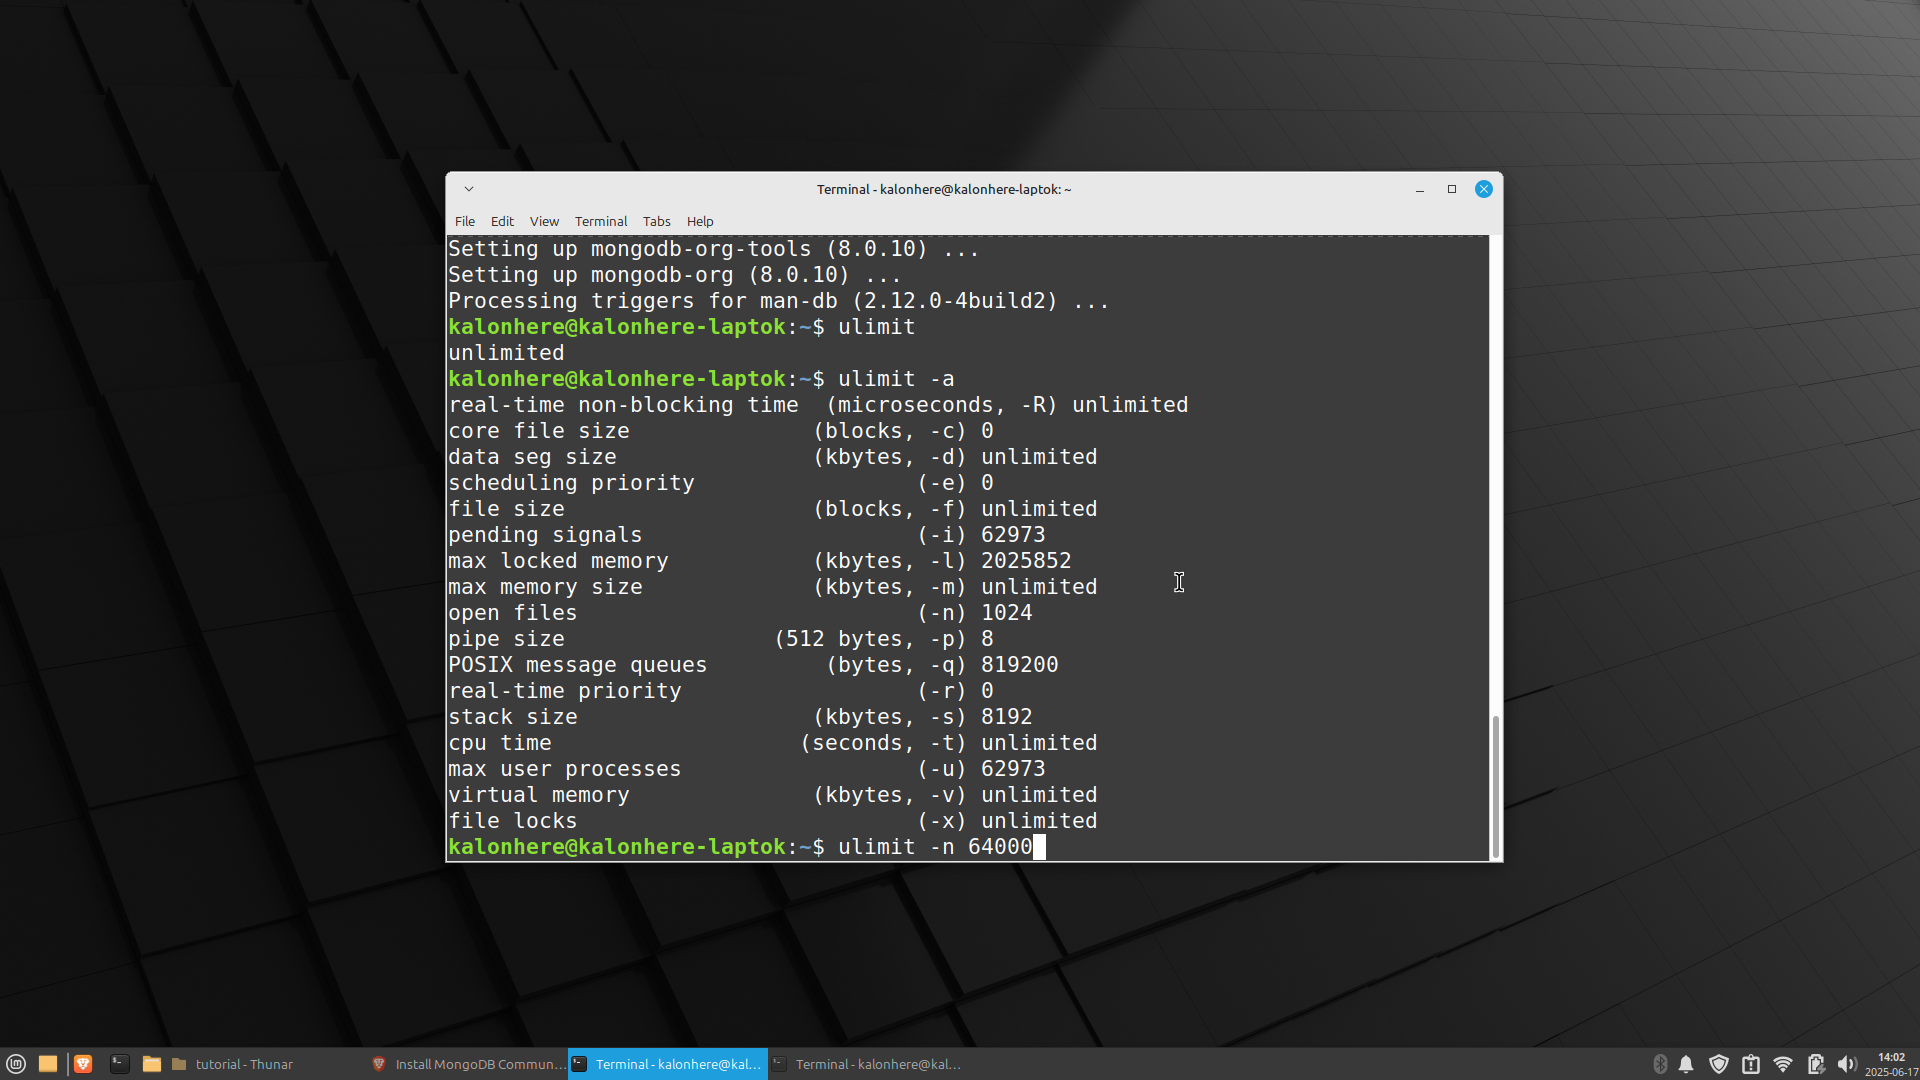
\includegraphics[width=\textwidth]{7_zmiana_ustawien_dotyczacych_plikow.png}
			\caption{Zwiększenie limitu otwartych plików z 1024 do 64000}
		\end{figure}

\newpage
		\begin{figure}[!ht]
			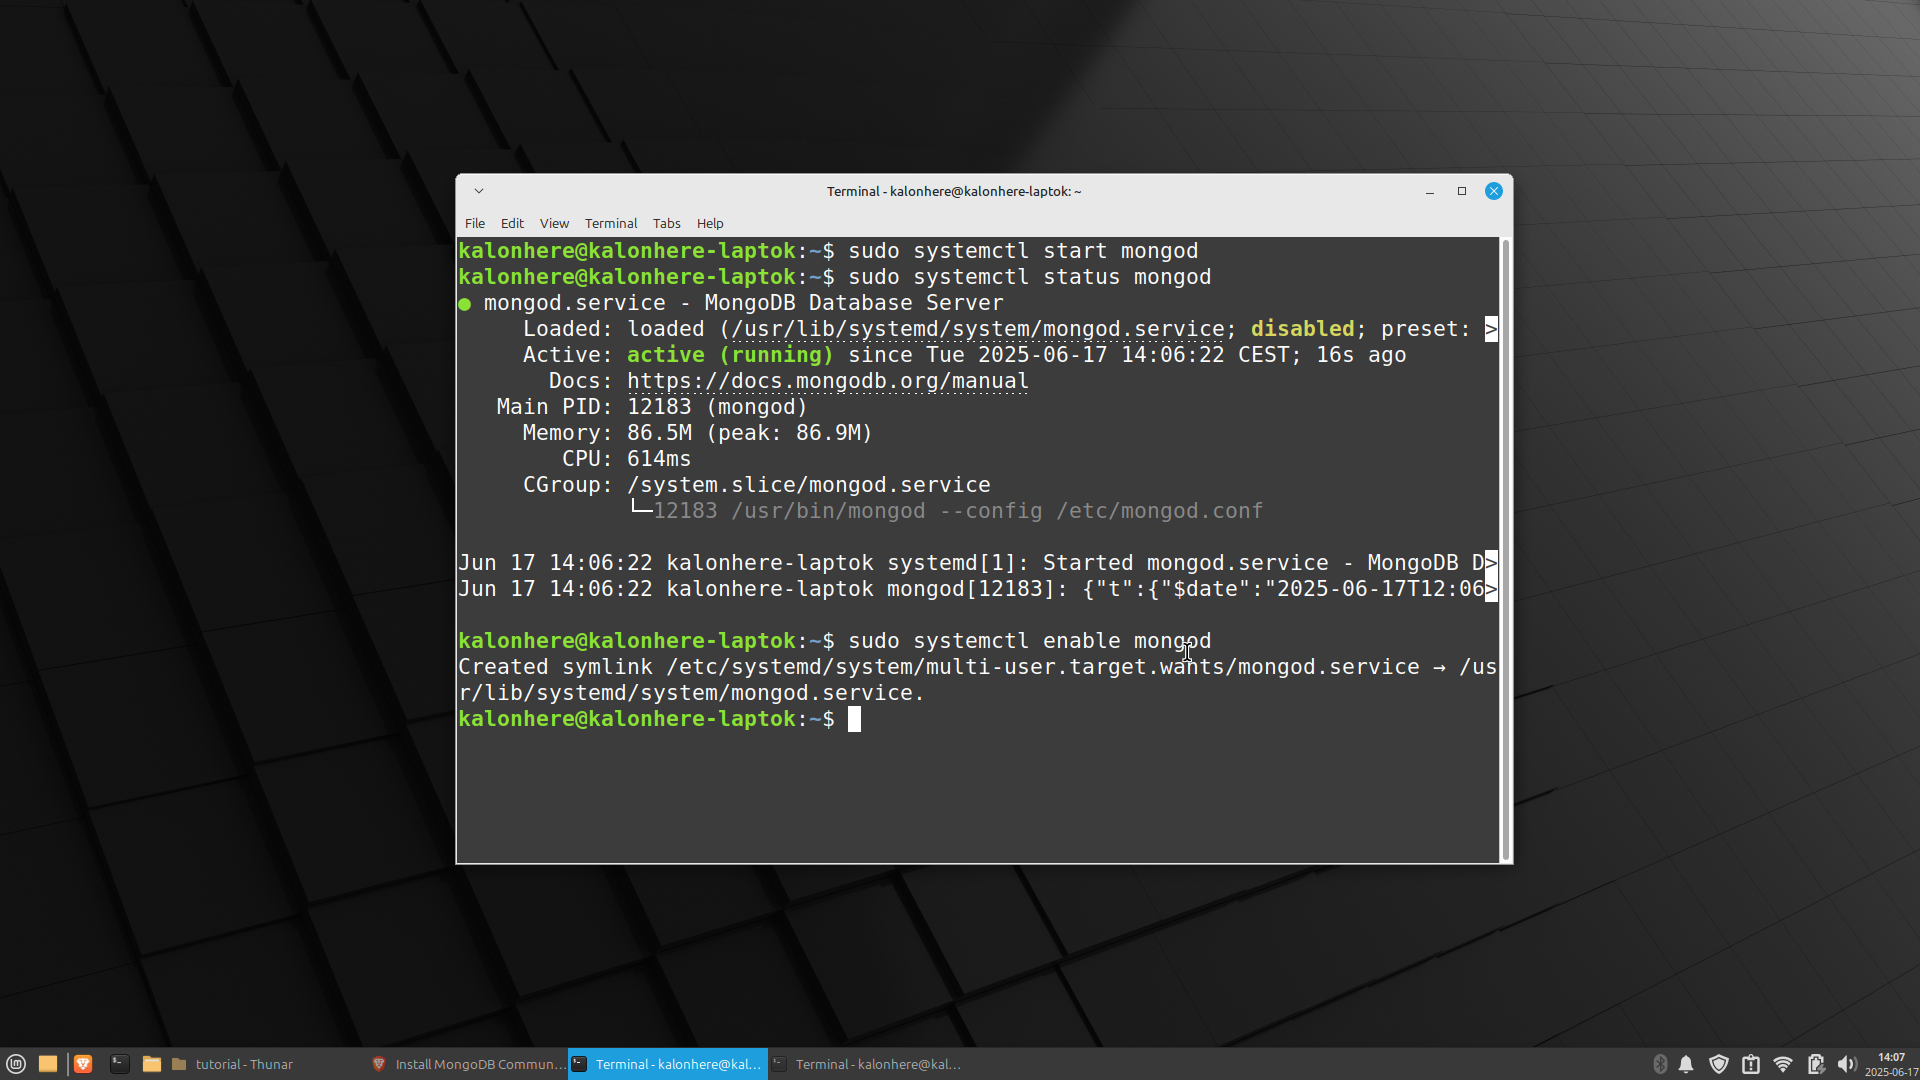
\includegraphics[width=\textwidth]{8_uruchomienie_sprawdzenie_i_aktywacja_autouruchamiania_mongodb.png}
			\caption{Uruchomienie MongoDB, sprawdzenie statusu i włączenie autouruchamiania}
		\end{figure}
\section{Lista zapytań po polsku}
	\begin{enumerate}
		\item  Wybierz państwo którego nazwa kończy się na "a" i ma najwięcej odkryć z fizyki
		\item Znajdź najstarsze i najmłodsze odkrycie z USA z biologii
		\item Znajdź państwa które mają odkrycia z biologii po 1960 roku
		\item Znajdź średnią liczbę wszystkich odkryć na państwo w każdym kontynencie
		\item  Wypisz dziedzine w której każde państwo z europy dokonało najwięcej odkryć
		\item  Wypisz średnią liczbę odkryć na naukowca z każdego kontynetu
		\item  Znajdź państwo z największą średnią liczbą odkryć na kilometr kwadratowy
		\item Znajdź miasto z którego pochodzi najwięcej fizyków
	\end{enumerate}

\newpage
\section{Zapytania w MongoDB}
	\subsection{Zapytanie 1}
		\begin{figure}[!ht]
			\begin{center}
				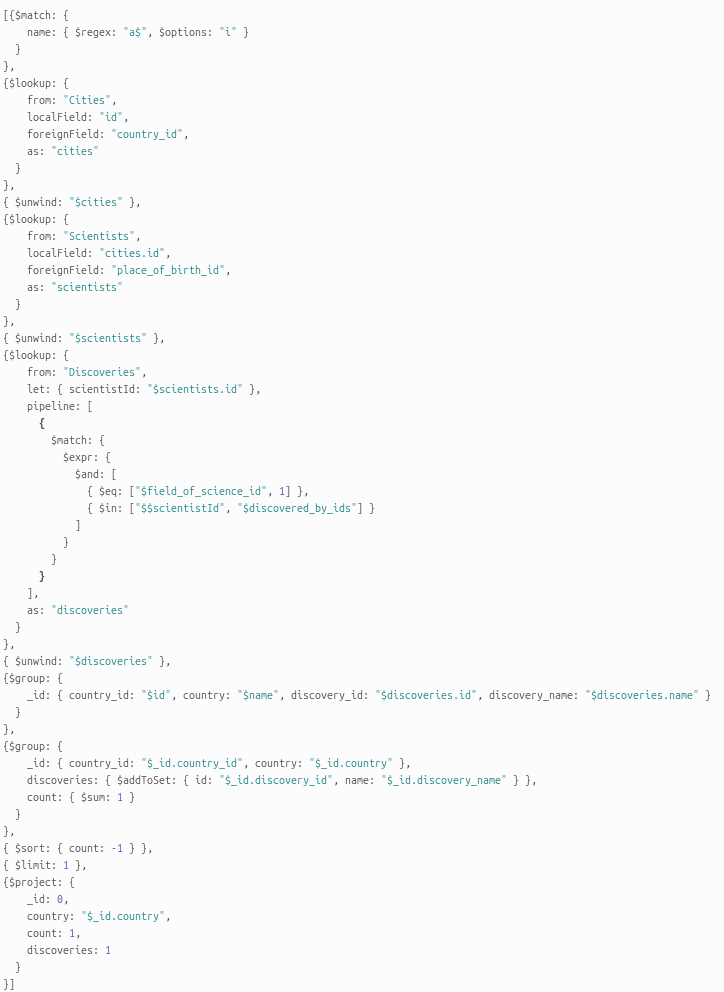
\includegraphics[width=400px]{m1.png}
			\end{center}
		\end{figure}

\newpage
	\subsection{Zapytanie 2}
		\begin{figure}[!ht]
			\begin{center}
				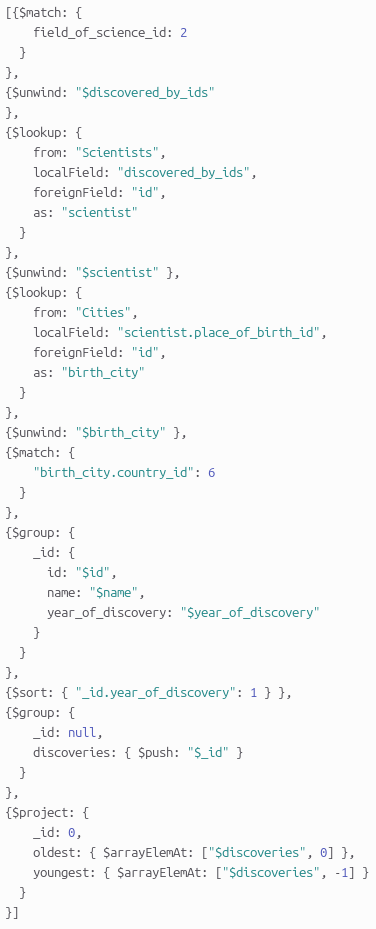
\includegraphics[width=230px]{m2.png}
			\end{center}
		\end{figure}

\newpage
	\subsection{Zapytanie 3}
		\begin{figure}[!ht]
			\begin{center}
				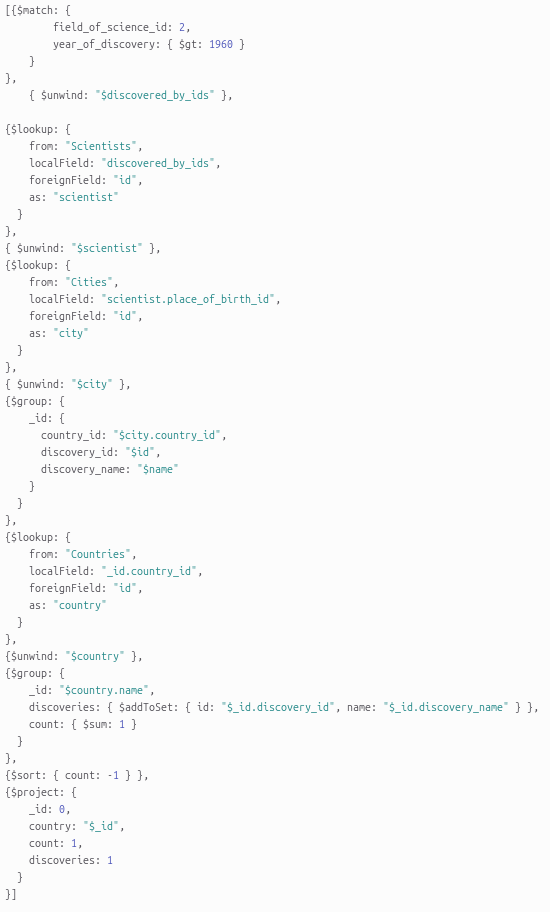
\includegraphics[width=350px]{m3.png}
			\end{center}
		\end{figure}

\newpage
	\subsection{Zapytanie 4}
		\begin{figure}[!ht]
			\begin{center}
				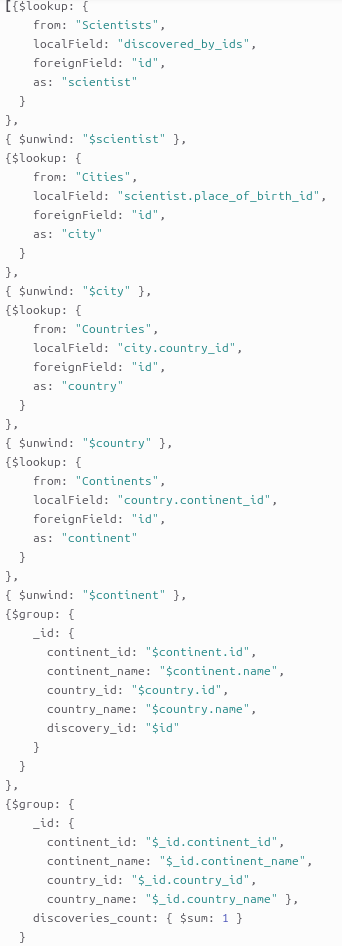
\includegraphics[width=200px]{m4_1.png}
			\end{center}
		\end{figure}

\newpage
		\begin{figure}[!ht]
			\begin{center}
				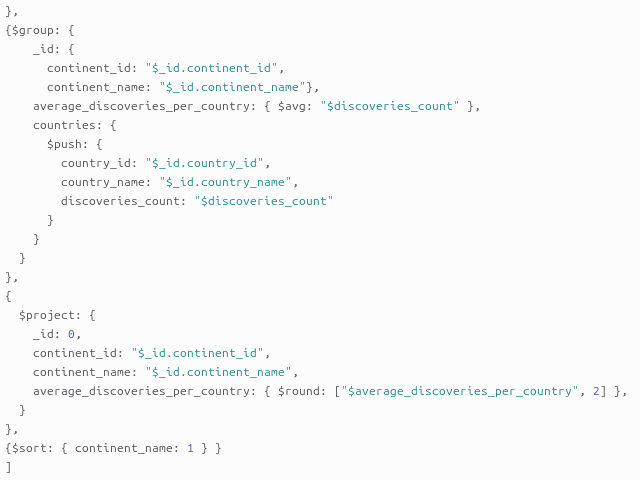
\includegraphics[width=350px]{m4_2.png}
			\end{center}
		\end{figure}

\newpage
	\subsection{Zapytanie 5}
		\begin{figure}[!ht]
			\begin{center}
				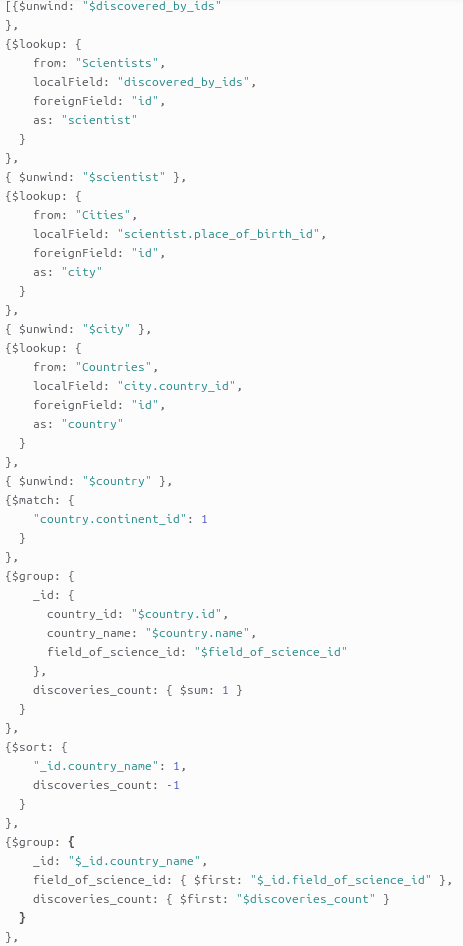
\includegraphics[width=250px]{m5_1.png}
			\end{center}
		\end{figure}

\newpage
		\begin{figure}[!ht]
			\begin{center}
				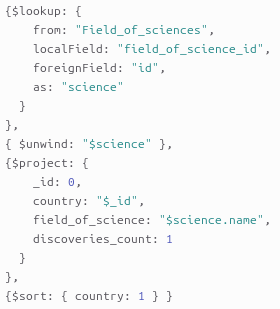
\includegraphics[width=250px]{m5_2.png}
			\end{center}
		\end{figure}


\newpage
	\subsection{Zapytanie 6}
		\begin{figure}[!ht]
			\begin{center}
				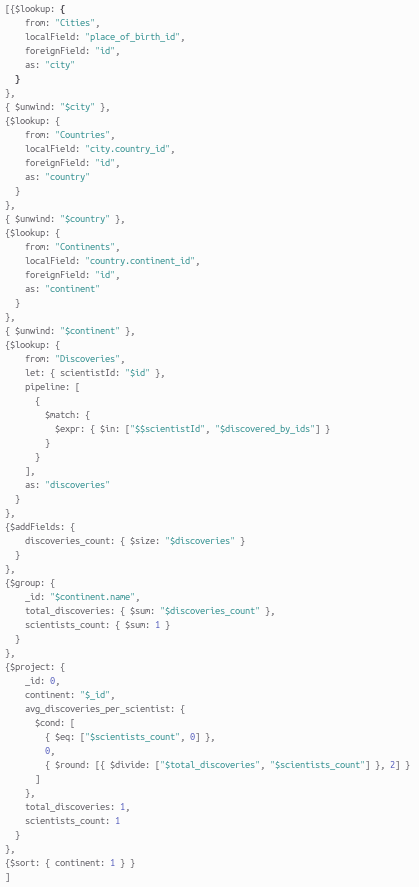
\includegraphics[width=250px]{m6.png}
			\end{center}
		\end{figure}

\newpage
	\subsection{Zapytanie 7}
		\begin{figure}[!ht]
			\begin{center}
				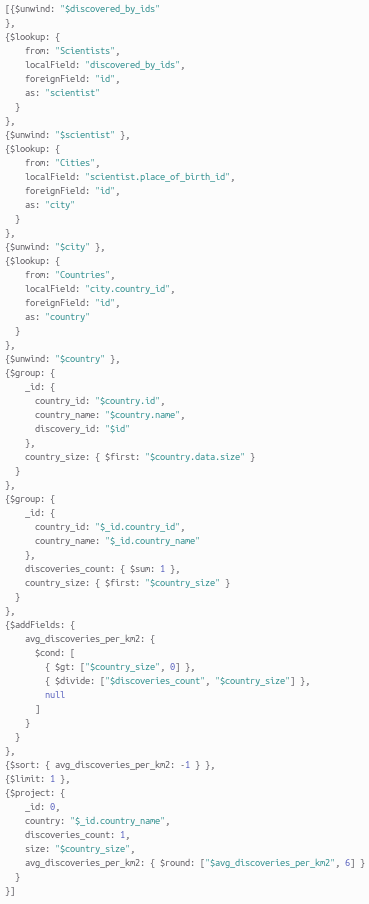
\includegraphics[width=230px]{m7.png}
			\end{center}
		\end{figure}

\newpage
	\subsection{Zapytanie 8}
		\begin{figure}[!ht]
			\begin{center}
				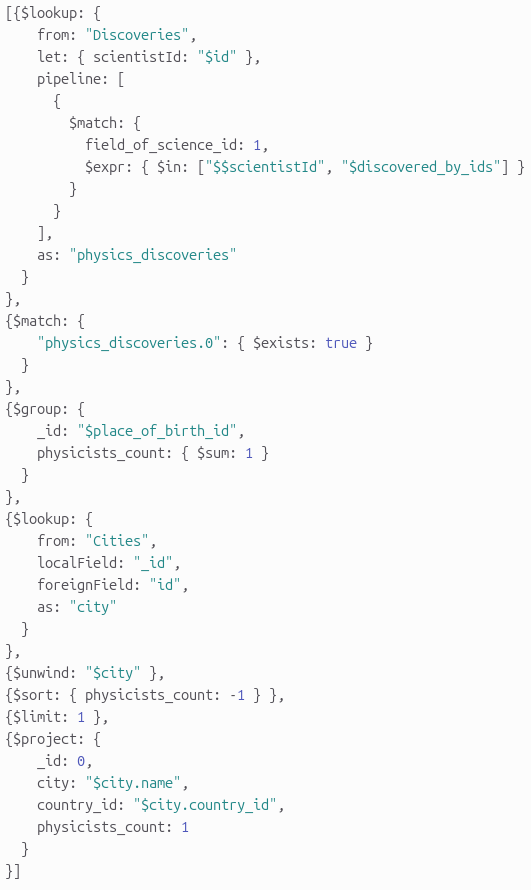
\includegraphics[width=250px]{m8.png}
			\end{center}
		\end{figure}

\newpage
\section{Zapytania w PostgreSQL}
	mnkln
\section{Zapytania w PostgreSQL w JSONB}
	faafefe

\newpage
\section{Porównanie czasowe zapytań}
	Po wykonaniu każdego zapytania odpowiednio, otrzymaliśmy następujące wyniki:
	\begin{table}[!ht]
	\begin{center}
		\begin{tabular}{ccccc}
			\toprule
			Zapytanie & MongoDB & PostreSQL-JSONB & PostrgreSQL &  \\
			\midrule
			1         & 22ms    &                 &             &  \\
			\midrule
			2         & 4ms     &                 &             &  \\
			\midrule
			3		  & 1ms     &                 &             &  \\
			\midrule
			4		  & 41ms    &                 &             &  \\
			\midrule
			5		  & 49ms    &                 &             &  \\
			\midrule
			6		  & 54ms    &                 &             &  \\
			\midrule
			7		  & 70ms    &                 &             &  \\
			\midrule
			8		  & 42ms    &                 &             &  \\
			\bottomrule
		\end{tabular}
	\end{center}
	\end{table}
\section{Uwagi końcowe}
	\begin{itemize}
		\item Brak udokumentowania procesu instalacji MongoDB Compass - zapomnieliśmy
		\item Brak udokumentowania procesu importowania do MongoDB - jedno kliknięcie w MongoDB Compass
		\item Brak udokumentowania procesu importowania do PostgreSQL JSONB - proszę zrozumieć, Filip po tym będzie miał traumę
		\item Brak udokumentowania procesu importowania do PostgreSQL - proste wklejenie sql z pliku do pgAdmin
		\item Słabe/Bezsensowne zapytania czy JSONy - nie dostaliśmy akcepta na czas :c
		\item Cały projekt z plikami - https://github.com/Aleks-Zielinski/DB-Benchmark
	\end{itemize}

\end{document}